\chapter{Python Variables: Storing Information}

\section{Introduction: Real-Life Hook}

Students often track things in real life:  

\begin{itemize}
    \item Pocket money  
    \item Number of books read  
    \item Test scores  
\end{itemize}

In Python, a \textbf{variable} stores information so the program can use it. Variables are like labeled boxes: you put a value inside, and you can change it anytime.

\section{Concept: Variables in Python}

\begin{definition}{Variable}
A \textbf{variable} is a name that refers to a value stored in the computer’s memory. 
\end{definition}

\subsection{Creating a Variable}

In Python, we can assign a value to a variable using the equal sign:

\begin{verbatim}
age = 15
name = "Rafi"
favorite_subject = "Math"
\end{verbatim}

\subsection{Rules for Naming Variables}

\begin{itemize}
    \item Cannot start with a number: \texttt{1age} $\times$  
    \item Can contain letters, numbers, and underscores: \texttt{age1} $\checkmark$, \texttt{my\_name} $\checkmark$  
    \item Cannot contain spaces or symbols: \texttt{my name} $\times$  
    \item Names are case-sensitive: \texttt{name} $\neq$ \texttt{Name}  
\end{itemize}

\section{Using Variables in Python}

Variables can be used in programs for calculations and display:

\begin{verbatim}
# Pocket money example
total_money = 1000
spent = 400
remaining = total_money - spent
print("Remaining money:", remaining)
\end{verbatim}

Output:

\begin{verbatim}
Remaining money: 600
\end{verbatim}

\section{Step-by-Step Diagram: Python Variable Flow}

\begin{center}
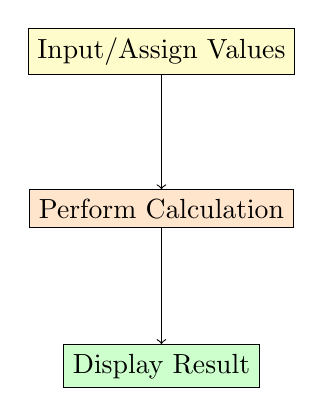
\begin{tikzpicture}[node distance=2cm]
\node (input) [draw, rectangle, fill=yellow!20] {Input/Assign Values};
\node (process) [draw, rectangle, fill=orange!20, below of=input] {Perform Calculation};
\node (output) [draw, rectangle, fill=green!20, below of=process] {Display Result};
\draw[->] (input) -- (process);
\draw[->] (process) -- (output);
\end{tikzpicture}
\end{center}

\section{Updating Variables}

Variables can change as the program runs:

\begin{verbatim}
score = 10
score = score + 5   # Update: score is now 15
print("New Score:", score)
\end{verbatim}

\section{Mini-Project: Python Self-Introduction Using Variables}

Write a program that stores your name, age, and favorite hobby in variables and prints a self-introduction:

\begin{verbatim}
# My self-introduction
name = "Amina"
age = 15
hobby = "painting"

print("Hello! My name is", name)
print("I am", age, "years old")
print("My favorite hobby is", hobby)
\end{verbatim}

Output:

\begin{verbatim}
Hello! My name is Amina
I am 15 years old
My favorite hobby is painting
\end{verbatim}

\section{Key Concepts}

\begin{itemize}
    \item A variable stores information in memory.
    \item Python variables can store numbers, text (strings), or boolean values.
    \item Variables can be updated anytime in a program.
    \item Correct naming of variables is important to avoid errors.
    \item Variables make programs flexible and reusable.
\end{itemize}

\section{End-of-Chapter Exercises}

\begin{exercise}{Very Short Questions}
\begin{enumerate}
    \item What is a variable in Python?
    \item Give three examples of variable names.
    \item Can variable names contain spaces?
\end{enumerate}
\end{exercise}

\begin{exercise}{Short Answer Questions}
\begin{enumerate}
    \item Write a Python program to store and display your favorite subject.
    \item Explain why variable names are case-sensitive.
    \item Give an example of updating a variable in Python.
\end{enumerate}
\end{exercise}

\begin{exercise}{Activity-Based Questions}
\begin{enumerate}
    \item Track your weekly pocket money using Python variables and calculate remaining money.
    \item Create variables for three hobbies and print them in one sentence.
    \item Modify the self-introduction program to include favorite subject and favorite food.
\end{enumerate}
\end{exercise}

\section{Teacher Notes}

\marginnote{
\textbf{Learning Objectives:} 
\begin{itemize}
    \item Students understand the concept of variables in Python.
    \item Students can create, use, and update variables.
    \item Students follow variable naming rules.
\end{itemize}

\textbf{Teaching Tips:} 
\begin{itemize}
    \item Use real-life examples like pocket money or books.
    \item Demonstrate updating variables in the Python shell.
\end{itemize}

\textbf{Assessment:} 
\begin{itemize}
    \item Observe students running variable programs.
    \item Check correctness of variable names and updates.
\end{itemize}
}